\documentclass[output=paper,colorlinks,citecolor=brown,
% hidelinks,
% showindex
]{langscibook}
\author{Joshua M. Griffiths\affiliation{The University of Texas at Austin}\orcid{0000-0001-6320-7365}}
\title{Augmenting the \textit{Projet Phonologie du Fran\c{c}ais Contemporain} corpus: A case study of schwa realization}
\abstract{Studies of French phonology have recently taken a methodological shift making use of data from large corpora, particularly since the advent of the \textit{Projet Phonologie du Fran\c{c}ais Contemporain} corpus \cite{pfc}. This corpus, coded specifically for schwa and liaison, two complex, variable hallmarks of French phonology, has not only been useful in studies of French phonology, but also in studies of phonological variation. While the PFC has been instrumental in shaping how phonology can be approached due to its coding system and sheer quantity of available data, the corpus is intended to be a first pass at the data and is purely descriptive. Here, I introduce a program that augments PFC schwa queries by offering a more granular insight into the phonological context of each schwa by indicating the sounds immediately to either side of the schwa as well as the word the schwa is found in. The augmented output is tested by analyzing the schwa-zero alternation in Meridional French, and it is found that a more granular means of annotating the phonological context of each schwa allows for the construction of stronger models of schwa realization.}
  
\IfFileExists{../localcommands.tex}{%hack to check whether this is being compiled as part of a collection or standalone
   % add all extra packages you need to load to this file

\usepackage{tabularx,multicol,multirow}
\usepackage{url}
\urlstyle{same}

\usepackage{listings}
\lstset{basicstyle=\ttfamily,tabsize=2,breaklines=true}

\usepackage{langsci-basic}
\usepackage{langsci-optional}
\usepackage{langsci-lgr}
\usepackage{langsci-gb4e}
%    \let\eachwordone=\it % Ch 14, 18

\usepackage{jambox}
\usepackage{subfigure}
\usepackage{tablefootnote}
\usepackage[nameinlink, noabbrev]{cleveref}
\crefname{enumi}{example}{examples}

\usepackage{bbding}
%\usepackage{linguex}
\usepackage{stmaryrd}

\usepackage{tipa}
\let\ipa\textipa
\usepackage{vowel}
\newcommand{\BlankCell}{}
\usepackage{ot-tableau}

\usepackage{forest}
\useforestlibrary{linguistics}
\usepackage[noeepic]{qtree}
\usepackage{pstricks, pst-xkey, pst-jtree}
\usepackage{tikz-qtree}
\usepackage{tikz-qtree-compat}
\usepackage{tree-dvips}

\usepackage{lastpage}
\usepackage{hyperref}
\usepackage{xltxtra}

\usepackage{ragged2e}
%\usepackage{subcaption}
\usepackage{floatrow}
\usepackage{float}

\usepackage[normalem]{ulem} % Pour les textes barrés
\usepackage{ifthen} 

\usepackage{todonotes}

   \newcommand*{\orcid}{}

\makeatletter
\let\theauthor\@author
\makeatother

\papernote{\scriptsize\normalfont
    \theauthor.
    \titleTemp. 
    To appear in: 
    Chad Howe and Pilar Chamorro and Timothy Gupton and Margaret Renwick.
    Theory, Data, and Practice: Selected papers from the 49th Linguistic Symposium on Romance Language
    Berlin: Language Science Press. [preliminary page numbering]
}

% Workaround for subscripts with capital letters
\newcommand{\capsub}[1]{\ensuremath{_\text{#1}}}

% Chapter 10: Table-like presentation within example environment
% classical latin > {*}late latin > old french  earlier > later   gloss
\newcommand{\montanoboxi}[7]{\parbox{2cm}{#1} > {#2}\parbox{2cm}{#3} > \parbox{1.5cm}{\textit{#4}} \parbox{1.2cm}{#5}\ > \parbox{1.2cm}{#6} \parbox{1.5cm}{#7}}
% {*}latin > earlier OF [ipa] > early OF   gloss
\newcommand{\montanoboxii}[6]{{#1}\parbox{1.9cm}{\textit{#2}} > \parbox{1.3cm}{\textit{#3}} \parbox{2cm}{#4} \parbox{2cm}{#5} \parbox{1.9cm}{#6}}

% Chapter 5
\newcommand{\redc}[1]{\textcolor{red}{#1}}
\newcommand{\bluec}[1]{\textcolor{blue}{#1}}
\newcommand{\ajout}[1]{\textcolor{blue}{#1}}
\newcommand{\ajoutplus}[1]{\textcolor{cyan}{#1}}

\newcommand{\hachure}[9]{
% Parametres :
% Coordonnees bas gauche (2 parametres) : (#1,#2)
% Coordonnees haut droit (2 parametres) : (#3,#4)
% Orientation : #5
%   1 : diagonale de pente 1
%  -1 : diagonale de pente -1
%   0 : horizontal
%   2 : vertical
% Nombre de pas horizontaux : #6
% Epaisseur du trait : #7
% Couleur : #8 (ex. green)
% Atténuation couleur : #9 (ex. 30)
\pgfmathsetmacro{\N}{#6-1}
\pgfmathsetmacro{\A}{#1}
\pgfmathsetmacro{\B}{#2}
\pgfmathsetmacro{\C}{#3}
\pgfmathsetmacro{\D}{#4}
\pgfmathsetmacro{\I}{(#3-#1)/#6}
\pgfmathsetmacro{\J}{(#4-#2)/#6}
\ifthenelse{\equal{#5}{1}}{
  \foreach \n in {0,...,\N}
    \foreach \m in {0,...,\N}
      {
        \pgfmathsetmacro{\X}{\A + ((0 + \n) * \I)}
        \pgfmathsetmacro{\Y}{\B + ((0 + \m) * \J)}
        \pgfmathsetmacro{\U}{\A + ((1 + \n) * \I)}
        \pgfmathsetmacro{\V}{\B + ((1 + \m) * \J)}
        \draw[#8!#9,#7] (\X, \Y)--(\U, \V);
      } 
  }{}
\ifthenelse{\equal{#5}{-1}}{
  \foreach \n in {0,...,\N}
    \foreach \m in {0,...,\N}
      {
        \pgfmathsetmacro{\X}{\A + ((1 + \n) * \I)}
        \pgfmathsetmacro{\Y}{\B + ((0 + \m) * \J)}
        \pgfmathsetmacro{\U}{\A + ((0 + \n) * \I)}
        \pgfmathsetmacro{\V}{\B + ((1 + \m) * \J)}
        \draw[#8!#9,#7] (\X, \Y)--(\U, \V);
      } 
  }{}
\ifthenelse{\equal{#5}{0}}{
  \foreach \n in {0,...,\N}
    \foreach \m in {0,...,\N}
      {
        \pgfmathsetmacro{\X}{\A + ((0 + \n) * \I)}
        \pgfmathsetmacro{\Y}{\B + ((0 + \m) * \J)}
        \pgfmathsetmacro{\U}{\A + ((1 + \n) * \I)}
        \pgfmathsetmacro{\V}{\B + ((0 + \m) * \J)}
        \draw[#8!#9,#7] (\X, \Y)--(\U, \V);
      } 
  }{}
\ifthenelse{\equal{#5}{2}}{
  \foreach \n in {0,...,\N}
    \foreach \m in {0,...,\N}
      {
        \pgfmathsetmacro{\X}{\A + ((0 + \n) * \I)}
        \pgfmathsetmacro{\Y}{\B + ((0 + \m) * \J)}
        \pgfmathsetmacro{\U}{\A + ((0 + \n) * \I)}
        \pgfmathsetmacro{\V}{\B + ((1 + \m) * \J)}
        \draw[#8!#9,#7] (\X, \Y)--(\U, \V);
      } 
  }{}
}

%Définition d'un pattern de type hachure
% \usetikzlibrary{patterns}
% \makeatletter
% \tikzset{hatch distance/.store in=\hatchdistance,hatch distance=5pt,hatch thickness/.store in=\hatchthickness,hatch thickness=5pt}

% \pgfdeclarepatternformonly[\hatchdistance,\hatchthickness]{north east hatch}% name
%     {\pgfqpoint{-\hatchthickness}{-\hatchthickness}}% below left
%     {\pgfqpoint{\hatchdistance+\hatchthickness}{\hatchdistance+\hatchthickness}}% above right
%     {\pgfpoint{\hatchdistance}{\hatchdistance}}%
%     {
%         \pgfsetcolor{\tikz@pattern@color}
%         \pgfsetlinewidth{\hatchthickness}
%         \pgfpathmoveto{\pgfqpoint{-\hatchthickness}{-\hatchthickness}}       
%         \pgfpathlineto{\pgfqpoint{\hatchdistance+\hatchthickness}{\hatchdistance+\hatchthickness}}
%         \pgfusepath{stroke}
%     }
% \pgfdeclarepatternformonly[\hatchdistance,\hatchthickness]{north west hatch}% name
%     {\pgfqpoint{-\hatchthickness}{-\hatchthickness}}% below left
%     {\pgfqpoint{\hatchdistance+\hatchthickness}{\hatchdistance+\hatchthickness}}% above right
%     {\pgfpoint{\hatchdistance}{\hatchdistance}}%
%     {
%         \pgfsetcolor{\tikz@pattern@color}
%         \pgfsetlinewidth{\hatchthickness}
%         \pgfpathmoveto{\pgfqpoint{\hatchdistance+\hatchthickness}{-\hatchthickness}}
%         \pgfpathlineto{\pgfqpoint{-\hatchthickness}{\hatchdistance+\hatchthickness}}
%         \pgfusepath{stroke}
%     }
% \makeatother
%~~~~~~~~~~~~~~~~~~~~~~~~~~~~~~~~~~~~~


% Chapter 7
\newcommand\pef[1]{(\ref{#1})}

\newcommand{\subscript}[1]{\textsubscript}

   %% hyphenation points for line breaks
%% Normally, automatic hyphenation in LaTeX is very good
%% If a word is mis-hyphenated, add it to this file
%%
%% add information to TeX file before \begin{document} with:
%% %% hyphenation points for line breaks
%% Normally, automatic hyphenation in LaTeX is very good
%% If a word is mis-hyphenated, add it to this file
%%
%% add information to TeX file before \begin{document} with:
%% %% hyphenation points for line breaks
%% Normally, automatic hyphenation in LaTeX is very good
%% If a word is mis-hyphenated, add it to this file
%%
%% add information to TeX file before \begin{document} with:
%% \include{localhyphenation}
\hyphenation{
anaph-o-ra
Dor-drecht
%FFI2016-76045-P-AEI/-MINEICO/-FEDE
}

\hyphenation{
anaph-o-ra
Dor-drecht
%FFI2016-76045-P-AEI/-MINEICO/-FEDE
}

\hyphenation{
anaph-o-ra
Dor-drecht
%FFI2016-76045-P-AEI/-MINEICO/-FEDE
}

    \bibliography{localbibliography}
    \togglepaper[23]
}{}

\begin{document}
\maketitle

\section{Introduction}
French phonology is well-known for a a high degree of variability, name due to the presence of a complicated schwa vowel and a variable sandhi phenomenon called \textit{liaison}. To offer new perspectives on these phenomena, approaches to French phonology have taken a methodological shift making use of large corpora. \citet{laks} argues broadly for corpus-based approaches to phonology stating that by nature of its questions, phonology should be a data-driven science and that the scale of the data offered through corpora allow simultaneously for a usage-based and grammatical approach to phonology. This bilateral approach may be advantageous in studying phonologically variable structures. \citet{durand9} echo this as they believe that corpora allow for a way to account for different manifestations of the heterogeneity of the linguistic signal as proposed by \citet{weinreich}.

The creation of the \textit{Projet phonologie du fran\c{c}ais contemporain corpus} \citep[PFC;]{pfc,pfc2,pfc3}\footnote{The corpus is accessible at http://www.projet-pfc.net/.} has been paramount in ushering in this new wave of corpus-based approaches to French phonology. Founded in 1999 by Jacques Durand, Bernard Laks, and Chantal Lyche, the PFC project is an international community of scholars devoted to the maintenance and use of a large database of spoken French from all over the world with the goal of studying French phonology, and providing authentic spoken French for the instruction of French as a foreign language. At the time of publication, the PFC contains over 1,500,000 words, more than 390 hours of spoken French, and over 450 speakers from 49 different points of investigation from all over the Francophone world including Europe; North America; the Maghreb, Sub-Saharan Africa, New Caledonia; and Guadeloupe. The impact of the PFC cannot be understated having given rise to several edited volumes \citep[i.e.]{detey,durand13,gess} in addition to numerous articles, doctoral theses, and book chapters. Furthermore, the PFC has inspired similar projects for English phonology \citet{pac}, Spanish phonology \citet{fec}, and L2 French phonology \citet{ipfc}.

No project is perfect, and while the size of and specificity afforded by the PFC have been instrumental in shaping how scholars have approached French phonology in recent years, there are inherent challenges tied to large corpora. In this paper, I introduce a program that increases the specificity of an initial PFC schwa query. In order to do so, I first review why the French schwa is of interest and how it is addressed in the PFC. Next, I introduce the schwa coding protocol in the PFC and discuss its advantages and disadvantages. In \sectref{sec:griffiths:pre} I describe the program that was written and what it adds to a schwa query. I follow this up with a case study comparing the results of a model predicting schwa realization in the initial query and a model predicting schwa realization from the annotated data. I conclude with the implications for this program and suggestions for how it can be implemented for further research.

\section{The French schwa}
\label{sec:griffiths:schwa}
In contemporary Modern French, the schwa -- also known as the \textit{e-muet} or \textit{e-caduc} -- is a mid-front, round vowel subject to multiple alternations with zero. Despite phonetic similarity to /ø/ and /œ/, the schwa is distinct in French, evidenced in part by the minimal pair in (\ref{ex:griffiths:mp}).
\begin{exe}
\ex\label{ex:griffiths:mp} \begin{xlist}
\ex\label{ex:griffiths:melon} \textit{(un) melon} /məlõ/ `(a) melon'
\ex\label{ex:griffiths:meulons} \textit{(nous) meulons} /mø.lõ/ `(we) grind'
\end{xlist}
\end{exe}
The schwa is subject to a limited phonological distribution as it is disallowed word-initially, in closed syllables, and in most stressed syllables. It is underlyingly licensed in most environments including as the nucleus of a word-initial syllable like in (\ref{ex:griffiths:initial}), word-medially as in (\ref{ex:griffiths:medial}), word-finally in (\ref{ex:griffiths:final}), and as the nucleus of the nine monosyllabic clitics listed in (\ref{ex:griffiths:clitic}).
\begin{exe}
\ex\label{ex:griffiths:initial} \textit{petit} /pə.ti/ $\rightarrow$ [pə.ti] $\sim$ [pti] `small'
\ex\label{ex:griffiths:medial} \textit{maintenant} /mɛ̃.tə.nɑ̃/ $\rightarrow$ [mɛ̃.tə.nɑ̃] $\sim$ [mɛ̃t.nɑ̃] `now'w'
\ex\label{ex:griffiths:final} \textit{Ecoute !} /e.ku.tə/ $\rightarrow$ [e.ku.tə] $\sim$ [e.kut] `Listen!'
\ex\label{ex:griffiths:clitic} \textit{ce} /sə/; \textit{de} /də/; \textit{je} /ʒə/; \textit{le} /lə/; \textit{me} /mə/; \textit{ne} /nə/; \textit{que} /kə/; \textit{se} /sə/; \textit{te} /tə/
\end{exe}
The most well-known feature of the schwa is its ability to alternate with zero, which appears to be in free variation. This alternation is complex as both variable deletion and variable epenthesis are possible. Contrast the example of deletion in (\ref{ex:griffiths:delete}) with the example of epenthesis in (\ref{ex:griffiths:epen}).
\begin{exe}
\ex\label{ex:griffiths:delete} \textit{maintenant} /mɛ̃.tə.nɑ̃/ $\rightarrow$ [mɛ̃.tə.nɑ̃] $\sim$ [mɛ̃t.nɑ̃] `now'
\ex\label{ex:griffiths:epen} \textit{Bonjour!} /bõ.ʒuʁ/ $\rightarrow$ [bõ.ʒuʁ] $\sim$ [bõ.ʒu.ʁə] `Hello!'
\end{exe}
The complexity of these alternations with zero in addition to the phonetic similarity with the distinct /œ,ø/ have led to the \textit{e-muet} being one of the most studied phenomena in phonology. The alternations with zero are rendered even more complex as they are influenced by a complex interplay of phonotactic, prosodic, and sociolinguistic factors. 


\subsection{Schwa in the PFC}
\label{sec:griffiths:schwa.pfc}
Corpus-based approaches have been called for as a means of analyzing the schwa-zero alternation  \citep{durand7,eychenne}, as well as the phonetic and sociolinguistic variability of the schwa \citep{lyche}. For example, \citet{durand} consider the case of word-final schwa in polysyllabic words in three varieties of French. Through an analysis of PFC data, they conclude that Meridional French distinguishes between /C\#/ and /Cə\#/, meaning that the words \textit{mer} (/mɛʁ/; `sea') and \textit{m\`ere} (/mɛʁə/; `mother') are phonologically distinct, while Northern French shows no distinction between /C\#/ and /Cə\#/, and the Basque Country is in the process of transitioning from the conservative Meridional to the more innovative Northern variety. \citeauthor{durand} believe that these conclusions would have been impossible to draw without the use of a corpus like the PFC. 

The PFC is designed specifically for the schwa, as each schwa and each site in which a schwa can possibly be epenthesized is tagged in the corpus. Each tag includes data concerning the phonological context of the schwa  as well as sociolinguistic metadata associated with the speaker that uttered it. Before being uploaded to the corpus, each recording is transcribed manually in Praat \citep{praat}. The audio is first transcribed orthographically, then in the IPA, and is finally segmented at multiple levels including levels for schwa and liaison. The transcription and annotation may not be cross-checked, and if they are validated by another researcher, no inter-rater reliability measures have been put in place. Part of the annotation process entails that each schwa is annotated with a protocol unique to the PFC. \citet{lyche} describes this protocol by first addressing some of the difficulties in defining schwa and how these difficulties and subsequent debates problematize the development of a descriptive, theoretically-neutral coding protocol.  For the PFC to classify a vowel as schwa, it must meet three criteria \citep[352]{lyche}:
\begin{enumerate}
\ex\label{ex:griffiths:2crit} It can be omitted altogether under variable conditions
\ex\label{ex:griffiths:2crit2} When realized, its usual quality is that of [\oe] or [\o]
\ex\label{ex:griffiths:2crit3} It normally corresponds to a written $e$ (excluding the digraph $eu$ anf the trigraph $eau$) not followed by a consonant within the same syllable
\end{enumerate}
Finally, to capture the possibility of epenthesis the PFC encodes all word-final pronounced consonants as potential schwa sites, whether or not a schwa is pronounced. This means that if the sequence \textit{il va} is realized as [il.va], then post-\textit{il} will be coded as a possible schwa site; however, if that same utterance were to be pronounced as [i.va], whereby the /l/ is elided, then the site will not be included as a possible schwa site.

This protocol is designed to be as theoretically neutral as possible and only serves to offer a preliminary description on which the researcher can build more complex analyses \citep[61]{pfc4}. The protocol encodes four factors tied to schwa realization, each of which is represented by a digit. The possible values of each factor are outlined in \tabref{tab:griffiths:proto}.
\begin{table}
\caption{PFC schwa coding protocol (\citeauthor{pfc}, \citeyear{pfc}, \citeyear{pfc2}, \citeyear{pfc3})}
\label{tab:griffiths:proto}
\begin{tabular}{lr}
  \lsptoprule
\textbf{First digit} & \textbf{Presence of schwa} \\ \midrule
Schwa not present & 0 \\
Schwa present & 1 \\
Uncertain schwa & 2 \\ \midrule
\textbf{Second digit} & \textbf{Position of schwa in the word} \\ \midrule
Monosyllabic word & 1 \\
First syllable of a polysyllabic word & 2 \\
Internal syllable of a polysyllabic word & 3 \\
Last syllable of a polysyllabic word & 4 \\
Metathesis & 5 \\ \midrule
\textbf{Third digit} & \textbf{Context to the left} \\ \midrule
Vowel to the left & 1 \\
Consonant to the left & 2 \\
First vowel in a prosodic phrase & 3 \\
Uncertain realization of a vowel to the left & 4 \\
Reduced consonant cluster & 5 \\ \midrule
\textbf{Fourth digit} & \textbf{Context to the right} \\ \midrule
Vowel to the right & 1 \\
Consonant to the right & 2 \\
Strong break and/or utterance final position & 3 \\
Weak break & 4 \\  \lspbottomrule
\end{tabular}
\end{table}

The first digit shows whether or not a schwa is phonetically realized. The second digit indicates the distribution of the schwa within the word, more specifically, whether schwa occurs in a monosyllabic word or where within a polysyllabic word it occurs. The third digit indicates the context preceding the schwa and the consonant that immediately precedes. Since a schwa must be realized with at least one consonant in its onset, a vowel annotated as XX2X occurs in the environment /...CCə.../ (i.e. \textit{une cerise} [yn.sə.ʁiz] `a cherry') and a vowel annotated as XX1X occurs in the context /...VCə.../ (i.e. \textit{la cerise} [la.sə.ʁiz] `the cherry'). The fourth digit indicates the context immediately following the schwa. As stated above, phonotactic, prosodic, and sociolinguistic factors play a role in the schwa-zero alternation. As simple as it may seem, the PFC protocol provides a great deal of information on these factors. For example, it has been understood that phonotactic constraints play a role in conditioning the schwa-zero alternation for well over a century. In particular the \textit{loi des trois consonnes} \citep{grammont} has been considered one of the most important constraints underpinning this alternation. This law is illustrated by contrasting the data in (\ref{ex:griffiths:l3c}).

\begin{exe}
\ex\label{ex:griffiths:l3c} \begin{xlist}
\ex\label{ex:griffiths:l2c} \textit{la petite} /la.pə.tit/ $\rightarrow$ [lap.tit] `the small one'
\ex\label{ex:griffiths:l3} \textit{cette petite} /sɛt.pə.tit/ $\rightarrow$ [sɛt.pə.tit] `that small one'
\end{xlist}
\end{exe}

While initially proposed as a Neogrammarian law, the three-consonant rule is understood to be more of a tendency than an actual law \citep{laks2}. The rule states that in the environment /...VC\_C/ like in (\ref{ex:griffiths:l2c}) a schwa can be deleted, but in the environment /...CC\_C/, as in (\ref{ex:griffiths:l3}), it must be maintained. The PFC protocol does capture this tendency; however, it is entirely possible that certain groups of consonants that surround the schwa may more likely to require maintenance than others.  Contrast the data in (\ref{ex:griffiths:l3c2}).
\begin{exe}
\ex\label{ex:griffiths:l3c2} \begin{xlist}
\ex\label{ex:griffiths:l3c2a} \textit{gouvernement} /gu.vɛʁ.nə.mɑ̃/ `government'
\ex\label{ex:griffiths:l3c2b} \textit{incroyablement} /ɛ̃.kʁwa.ja.blə.mɑ̃/ `incredibly'
\end{xlist}
\end{exe}
The resyllabification required by deletion of the schwa in (\ref{ex:griffiths:l3c2b}) would license a rising coda, in contrast with the falling coda licensed by schwa elision in (\ref{ex:griffiths:l3c2a}). It would seem that the schwa in (\ref{ex:griffiths:l3c2a}) would be more susceptible to deletion than the schwa in (\ref{ex:griffiths:l3c2b}). As it currently stands, the PFC schwa protocol would require a more precise means of annotating the context surrounding each schwa to shed light on the nuances captured by the contrast in (\ref{ex:griffiths:l3c2}).

\subsection{Challenges with the PFC schwa coding protocol}
\label{sec:griffiths:issues}
\citet{lyche} addresses some of the difficulty in developing any protocol specifically for schwa, and \citet{eychenne} discusses some of the shortcomings of the PFC schwa protocol in particular.  The first issue addressed by \citet[42]{eychenne} is the difficulty tied to concretely identifying a phonological object with this sort of protocol since phonological representations are abstract objects manifested concretely in an acoustic signal. When a phoneme is codified by a researcher, its representation is distorted as it is subject to the perception and bias of the researcher.  Furthermore, some coders may not agree on the identification of a particular token as a schwa.  \citeauthor{eychenne} provides his own anecdotal evidence in which speakers of Meridional French may identify an epenthesized schwa as an underlying schwa, coded as 1XXX. According to Eychenne, this can be attributed to the difference described earlier, in which Southerners maintain lexical, word-final schwas, whereas speakers of non-Meridional French, who lack word-final lexical schwa may hesitate to identify it as a schwa, and would therefore code it as 2XXX or an ``uncertain schwa."

Another issue brought to light by \citet[43]{eychenne} relates to discrepancies tied to phonological domains. Consider the case of the word \textit{parce que} /paʁsə kə/ (`because'). The definition of schwa employed by the PFC incorporates orthography. The inclusion of orthography when defining schwa requires that \textit{parce que} be treated as two individual words, but the PFC is inconsistent in how \textit{parce que} is coded. Querying the PFC for this word outputs 2078 tokens. The schwa in the first stem (\textit{parce}) is coded most often as a word-internal schwa (1823; 87.73\%), but it is also coded as a word-final schwa 254 times (12.22\%) and there is one token coded as a monosyllabic word.

While \citet{lyche} touts the simplicity of the  protocol as a positive, there are some challenges that result from this lack of specificity.  The third and fourth digits only specify pre- or post-consonantal, pre- or post-vocalic, or pre- or post-pausal contexts. This three-way distinction does not offer much insight into the conditioning environment of the schwa-zero alternation. Many studies that have made use of this protocol have done little to nothing in defining a more granular means of specifying the phonological context of the schwa such as the segment immediately preceding the schwa. Moreover, since the third digit is concerned with the segment preceding the onset of the schwa, nothing is known of the segment that immediately precedes it, and some studies have suggested that this segment does in fact play a role in schwa realization \cite{malecot}. This three-way distinction (C vs. V vs. \#) should be compared to a protocol that more granularly identifies the contexts surrounding the schwa and includes the immediately preceding segment. Another issue to address is the fact that all sites in which a schwa can be epenthesized are annotated as schwa regardless of whether or not a schwa is realized, like the following examples taken from the PFC.
\begin{exe}
\ex\label{ex:griffiths:possible} \begin{xlist} 
\ex\label{ex:griffiths:pour} \textit{pour}0412 \textit{v\'erifier} [puʁ.ve.ʁi.fje] `to verify'
\ex\label{ex:griffiths:saint} \textit{quel}0412 \textit{saint} [kɛl.sɛ̃]  `which saint'
\end{xlist}
\end{exe}
As there is neither an underlying nor epenthesized schwa present in the data in (\ref{ex:griffiths:possible}), some analyses making use of PFC data could be inaccurate if the researcher is unaware of their inclusion or is not meticulous in their own cleaning of the data.

\section{Augmenting a PFC query}
\label{sec:griffiths:pre}
For this case study, the PFC was queried for all present and absent schwas in the semi-structured and unstructured conversational tasks in Metropolitan French. Clitics and tokens with an uncertain schwa in the preceding syllable were excluded. This initial query output a total of 52,301 tokens distributed according to the criteria in \tabref{tab:griffiths:query}.

\begin{table}
\caption{Breakdown of initial PFC query by criterion $(n=52301)$}
\label{tab:griffiths:query}
\begin{tabular}{llrr} \lsptoprule
\textbf{Query tool} & \textbf{Criterion} & \textbf{Code} & \textbf{Total} \\ \midrule
Task & Guided conversation & g & 28819 \\
 & Unguided conversation & l & 23482 \\ \midrule
Schwa presence & Absent & 0 & 42516 \\
 & Present & 1 & 9785 \\ \midrule
Schwa distribution & Word-initial syllable & 2 & 3266 \\
 & Word-internal syllable & 3 & 3764 \\
 & Word-final syllable & 4 & 45271 \\ \midrule
Preceding context & Vowel to the left & 1 & 44238 \\
 & Consonant to the left & 2 & 6162 \\
 & Beginning of prosodic phrase & 3 & 284 \\
 & Reduced consonant cluster to the left & 5 & 1617 \\ \midrule
Following context & Vowel to the right & 1 & 11407 \\
 & Consonant to the right & 2 & 28446 \\
 & Strong break to the right & 3 & 6303 \\
 & Weak break to the right & 4 & 6145 \\  \lspbottomrule
\end{tabular}
\end{table}

If this query were to be taken at face value, it would seem that 81\% of schwas were deleted, 87\% of schwas were licensed word-finally, and 85\% of schwas were licensed after a sequence of VC; however, closer examination of the data found that these figures are inaccurate, primarily due to the inclusion of possible schwa tokens that do not contain a schwa like in (\ref{ex:griffiths:possible}). In order to clean and further specify the query, data were pre-processed in R \citep{r_core_team_r_2019}. The pre-processing program made use of text manipulation functions in Base-R as well as in the shiny \citep{shiny} and tidyverse \citep{tidyverse} packages taking advantage of the inclusion of orthography in defining the schwa.

First, the program identified the orthography of the lexical contexts immediately to either side of the schwa and the orthographic representations for the surrounding contexts was manually matched to their phonemic representations. For example, from a sequence coded as \textit{mainte1312nant} in the PFC, we would know that we have a phonetically realized, word-internal schwa in the environment /VC\_C/. However, the present program will tell us that this is schwa is preceded by /t/ and followed by /n/. These sounds were then tagged with their voicing value, manner of articulation, and these two values were combined to give a rough approximation of natural class of the sound (i.e. voiceless stop). There were some difficulties in constructing these lists that had to be accounted for. Let us reconsider the word \textit{parce que} as an example. This word appeared 1171 in this query. In the column that specifies the lexical context immediately to the left of the schwa (CG\_imm) almost all tokens $(n=1145)$ were transcribed as \textit{parce}; however, 2 tokens were transcribed as \textit{par}, and 24 were transcribed as \textit{parc}. While the presence of neither \textit{par} nor \textit{parc} was significant, their inclusion is problematic for a program reliant on text. Another problem is posed by the rather opaque orthography of French.  For example, the words \textit{ville} /vi.lə/ (`city') and \textit{famille} /fa.mi.jə/ (`family') both end in an orthographic sequence of $<ille>$; therefore, each one had to be identified separately.

Recall that the PFC encodes all possible schwa sites even if a schwa is not realized; therefore, once the contexts surrounding the schwa were identified, all \textit{possible} schwa sites in which a schwa was not epenthesized (i.e. \textit{alors0413}) were removed. This was done by specifying all word-final absent schwas in words that did not end in a graphemic $<e>$. This removed 16281 tokens -- or 31\% of the initial query. The results of a McNemar test revealed that the elimination of these tokens alone resulted in a significant difference in schwa realization between the initial query and any pre-processed subset that would follow suit $(\chi^2=537.14;df=1;p<0.001)$.

Next, any instance of the full vowel /ø/ that had been misidentified as schwa was eliminated. This resulted in the elimination of 71 tokens. Almost all of the misidentified instance of /ø/ were in the word \textit{peut-\^etre} (`maybe'; $n=64$), but misidentified /ø/ vowels were also found in the words \textit{neurologique} (`neurological'); \textit{d\'ejeuner} (`to eat lunch'); and \textit{engueuler} (`to tell somebody off.') In order to avoid conflation of the phonetically similar hesitation vowel with the schwa, any schwa in the immediate presence of the hesitation vowel transcribed as \textit{euh} was also eliminated $(n=3476)$.

Finally, forty-nine tokens were eliminated if either the preceding or following context was unable to be identified by the neither the initial researcher nor the current program. This left a total of 32424 (61.99\%) tokens presented in \tabref{tab:griffiths:query2}. With these remaining tokens, the information in the PFC that specifies the lexical context to either side of the schwa was used to specify the word containing schwa (ie. \textit{dev} $+$ \textit{nir} \textit{dev}-ə-\textit{nir} `to become').

\begin{table}
\caption{Breakdown of remaining tokens by criterion $(n=32424)$}
\label{tab:griffiths:query2}
\begin{tabular}{llrr}  \lsptoprule
\textbf{Query tool} & \textbf{Criterion} & \textbf{Code} & \textbf{Total} \\ \midrule
Task & Guided conversation & g & 17911 \\
 & Unguided conversation & l & 14513 \\ \midrule
Schwa presence & Absent & 0 & 24044 \\
 & Present & 1 & 8380 \\ \midrule
Schwa distribution & Word-initial syllable & 2 & 3201 \\
 & Word-internal syllable & 3 & 3750 \\
 & Word-final syllable & 4 & 25473 \\ \midrule
Preceding context & Vowel to the left & 1 & 26196 \\
 & Consonant to the left & 2 & 5309 \\
 & Beginning of prosodic phrase & 3 & 215 \\
 & Reduced consonant cluster to the left & 5 & 704 \\ \midrule
Following context & Vowel to the right & 1 & 6095 \\
 & Consonant to the right & 2 & 24060 \\
 & Strong break to the right & 3 & 2626 \\
 & Weak break to the right & 4 & 3243 \\  \lspbottomrule
\end{tabular}
\end{table}

\section{A case study: Meridional French}
\label{sec:griffiths:analysis}
In order to test if the program described above is warranted, the subset of data from Meridional (Southern) French $(n=10484)$ were fit to generalized linear mixed-effects models using the lmerTest package in R \citep{kuznetsova}. The Meridional French data were chosen because the presence of a word-final schwa in this variety is less controversial than in other varieties, following from the work of \citet{durand2} and \citet{durand}. The first GLMER model predicted schwa realization from the three phonological factors encoded for in the PFC (preceding context, following context, and distribution in the word) in addition to the two random effects for word and speaker. The results of this model are presented in \tabref{tab:griffiths:results}.

\begin{table}
\caption{Model predicting schwa realization from PFC predictors}
\label{tab:griffiths:results}
\begin{tabular}{lrrrr}
\lsptoprule
Log likelihood & -4190.20 &  &  &  \\
Deviance & 8380.50 &  &  &  \\ \midrule
\textbf{Fixed effects} & \textbf{Estimate} & \textbf{Std. error} & $Z$ & $Pr(>|z|)$ \\ \midrule
(Intercept) & 3.254 & 0.247 & 13.164 & $<0.001$ \\
Cons. to left & 1.445 & 0.126 & 11.442 & $<0.001$ \\
First vowel in phrase & 0.127 & 0.471 & 0.269 & 0.790 \\
Reduced CC to left & -2.756 & 0.427 & -6.454 & $<0.001$ \\
Vowel to right & -3.977 & 0.130 & -30.588 & $<0.001$ \\
Strong break to right & 1.205 & 0.104 & 11.634 & $<0.001$ \\
Weak break to right & 1.110 & 0.126 & 9.139 & $<0.001$ \\
Word-internal syllable & -2.275 & 0.227 & -10.024 & $<0.001$ \\
Word-final syllable & -2.826 & 0.197 & -14.353 & $<0.001$ \\ \midrule
\textbf{Random effects }& $\sigma^2$ & $\sigma$ &  &  \\ \midrule
Word & 1.365 & 1.168 &  &  \\
Speaker & 2.153 & 1.467 &  &  \\ \lspbottomrule
\end{tabular}
\end{table}

The relative risk of schwa realization given the significant predictors in \tabref{tab:griffiths:results} is illustrated in \figref{fig:griffiths:clean.graph1}.

\begin{figure}

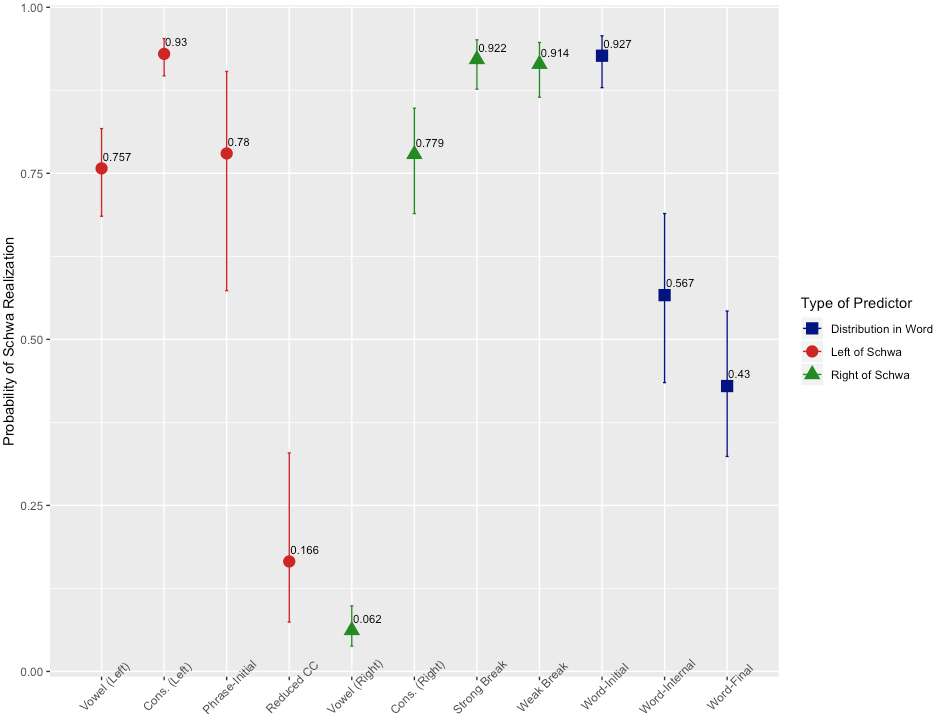
\includegraphics[scale=.4]{../figures/griffiths_clean-graph1.png}
\caption{Predictors of Schwa Realization in First Model}
\label{fig:griffiths:clean.graph1}
\end{figure}
It was found that the overall most likely context for schwa realization was in the /CCə.../ condition $(p=0.930)$ as in (\ref{ex:griffiths:l3c1}).
\begin{exe}
\ex\label{ex:griffiths:l3c1} \textit{Angleterre} /ɑ̃.glə.tɛʁ/ $\rightarrow$ [ɑ̃.glə.tɛʁ] `England'
\end{exe}
On the other hand, the least likely context for schwa realization $(p=0.062)$ was the pre-vocalic condition.
\begin{exe}
\ex\label{ex:griffiths:prev1} \textit{elle a} /ɛ.lə a/ $\rightarrow$ [ɛ.la] `she has'
\end{exe}
As for the distribution of the schwa within the word, realization was most likely to occur in the word-initial syllable $(p=0.927)$ like in (\ref{ex:griffiths:winit1}).
\begin{exe}
\ex\label{ex:griffiths:winit1} \textit{depuis} /də.pɥi/ $\rightarrow$ [də.pɥi] `since'
\end{exe}
The results of this model are largely unsurprising, but it is difficult to interpret anything beyond the results of this model with the query in its present format. Further investigation towards a more granular understanding of the schwa-zero alternation would require analysis of the transcriptions to either side of the schwa which would quickly become time-intensive and laborious.

Another GLMER model, predicting schwa realization from the same predictors as the model in \tabref{tab:griffiths:results} but also included the manner of articulation of the segment immediately preceding the schwa was constructed next.  Not only did the augmented model offer a more complete picture of the phonological environment surrounding the schwa, but the results of a likelihood ratio test assessing the goodness-of-fit of the two models found that the augmented model fit the data better $(\chi^2 = 38.384; df = 4; p <0.001)$. This improvement was reinforced by a comparison of the Akaike Information Criterion \citep[AIC;]{akaike} of each model. The simpler model $(AIC_1=8402.49)$ had a higher AIC value than the augmented model $(AIC_2=8370.11; \Delta_{AIC}=-32.38)$ further reinforcing that the inclusion of the preceding segment was better able to explain the schwa-zero alternation than its exclusion. The results of the augmented model are presented in \tabref{tab:griffiths:results2}, and the relative risk of schwa realization given the significant predictors in \tabref{tab:griffiths:results2} is illustrated in \figref{fig:griffiths:clean.graph2}.

\begin{table}
\caption{Model predicting schwa realization from augmented output}
\label{tab:griffiths:results2}
\begin{tabular}{lrrrr}
\midrule
Log likelihood & -4171.10 &  &  &  \\
Deviance & 8342.10 &  &  &  \\ \midrule
\textbf{Fixed effects} & \textbf{Estimate} & \textbf{Std. error} & $Z$ & $Pr(>|z|)$ \\ \midrule
(Intercept) & 3.705 & 0.261 & 14.205 & $<0.001$ \\
Cons. to left & 1.396 & 0.127 & 11.017 & $<0.001$ \\
First vowel in phrase & 0.090 & .471 & 0.191 & 0.850 \\
Reduced CC to left & -2.747 & .425 & -6.455 & $<0.001$ \\
Vowel to right & -3.968 & 0.130 & -30.589 & $<0.001$ \\
Strong break to right & 1.207 & 0.103 & 11.690 & $<0.001$ \\
Weak break to right & 1.120 & 0.121 & 9.237 & $<0.001$ \\
Word-internal syllable & -2.265 & 0.225 & -10.064 & $<0.001$ \\
Word-final syllable & -2.817 & 0.196 & -14.404 & $<0.001$ \\
Preceding fricative & -0.776 & 0.134 & -5781 & $<0.001$ \\
Preceding liquid & -0.568 & 0.124 & -4.565 & $<0.001$ \\
Preceding nasal cons. & -0.600 & 0.155 & -3.848 & $<0.001$ \\ \midrule
\textbf{Random effects} & $\sigma^2$ & $\sigma$ &  &  \\ \midrule
Word & 1.276 & 1.130 &  &  \\
Speaker & 2.162 & 1.471 &  &  \\ \midrule
\end{tabular}
\end{table}
\todo[inline]{Did you mean -5.781 for std. error for preceding fricative?}

\begin{figure}

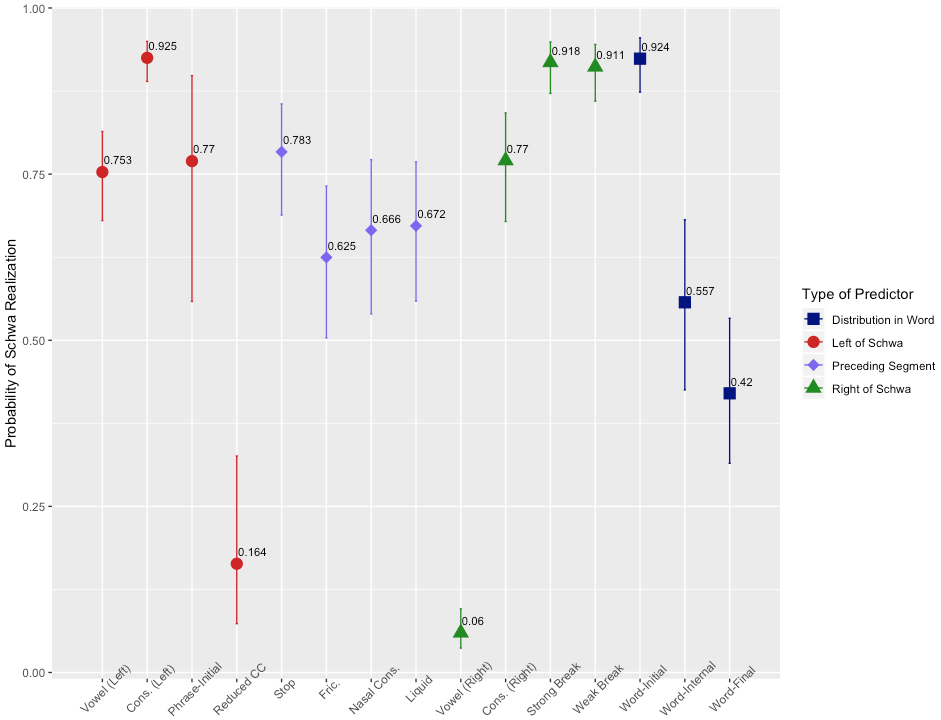
\includegraphics[scale=.4]{../figures/griffiths_clean-graph2.png}
\caption{Predictors of Schwa Realization in Expanded Model}
\label{fig:griffiths:clean.graph2}
\end{figure}

A random forest model, the results of which are presented in \figref{fig:griffiths:importance}, was grown assessing the relative importance of the four factors in predicting the schwa-zero alternation.

\begin{figure}

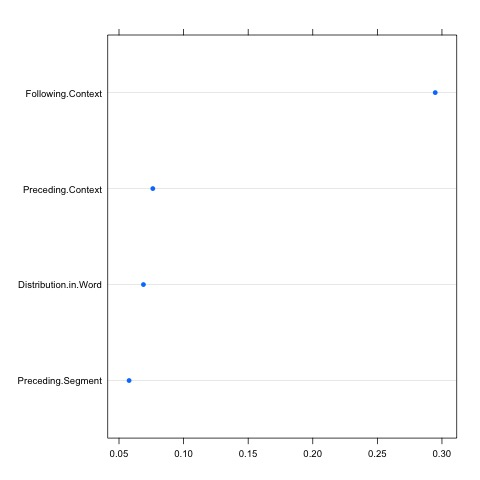
\includegraphics[scale=.7]{../figures/griffiths_importance.jpg}
\caption{Relative Importance of Factors Predicting the Schwa-Zero Alternation}
\label{fig:griffiths:importance}
\end{figure}

While the model found that the preceding segment was the least important predictor in predicting the schwa-zero alternation, the results of a post-hoc Wald test found that it was a significant predictor $(\chi^2=42.47 ; df =4 ; p <0.001)$, and as evidenced above, its removal resulted in a weaker model. The random forest also indicated that the most important factor in predicting the schwa-zero alternation is the context to the right of the schwa indicating that the variation may largely be driven by the changes in what follows word-final schwa, which as shown in \tabref{tab:griffiths:query2} made up the majority of tokens.

By and large, the patterns predicted by the two models were similar; however, the augmented model shed light on what role the preceding segment can play in conditioning the schwa-zero alternation: schwa is most likely to be realized before a stop, and most likely to be deleted before a fricative. An effect of fricatives as facilitators of schwa deletion has been suggested before, but precisely which fricatives condition deletion are not known \citep{rialland}. To better understand the differences between the fricatives and the role they play in conditioning schwa realization, let us assume the featural representation for the natural class of fricatives in (\ref{ex:griffiths:5fricn2}).

\begin{exe}
\ex\label{ex:griffiths:5fricn2} $\begin{bmatrix}
+\text{cons}\\
+\text{cont}\\
-\text{son}
\end{bmatrix}$
\end{exe}
The specifications for fricatives can be observed in (\ref{ex:griffiths:5fricn3}).
\begin{exe}
\ex\label{ex:griffiths:5fricn3} \ \\ \begin{tabular}{cccc}
 & [cor] & [ant] & [voi] \\ \cline{2-4} 
\multicolumn{1}{c|}{f} & - & + & - \\
\multicolumn{1}{c|}{v} & - & + & + \\
\multicolumn{1}{c|}{s} & + & + & - \\
\multicolumn{1}{c|}{z} & + & + & + \\
\multicolumn{1}{c|}{ʃ} & + & - & - \\
\multicolumn{1}{c|}{ʒ} & + & - & +
\end{tabular}
\end{exe}
\todo[inline]{Should this and (18) be converted to normal tables?}

The subset of schwas that followed fricatives were annotated for the featural specifications in (\ref{ex:griffiths:5fricn3}),  and significant differences at the level of $p<0.001$ were found along all features. In particular, it was found that schwa deletion was significantly more common after fricatives specified as [$+$coronal; $+$anterior; $-$voice]; thus, it would seem that in Meridional French, the effect of fricatives on schwa deletion can be attributed to the phoneme /s/, which was also the most common fricative in the corpus (1465 of 2248 tokens or 65\%). An example of a schwa in this context can be observed in (\ref{ex:griffiths:schwas}).
\begin{exe}
    \ex\label{ex:griffiths:schwas} \textit{la semaine} /la sə.mɛn/ $\rightarrow$ [la.sə.mɛn] `the week' (Speaker 13alg1)
\end{exe}

This same  process could be applied to the natural class of stops, which were found to be the segments most likely to condition schwa realization. Consider the featural representation of stops in (\ref{ex:griffiths:5stop2}).
\begin{exe}
\ex\label{ex:griffiths:5stop2} $\begin{bmatrix}
+\text{cons}\\
-\text{cont}\\
-\text{son}
\end{bmatrix}$
\end{exe}
The specifications for stops is shown in (\ref{ex:griffiths:5stop3}).
\begin{exe}
\ex\label{ex:griffiths:5stop3} \ \\ \begin{tabular}{cccc}
 & [cor] & [ant] & [voi] \\ \cline{2-4} 
\multicolumn{1}{c|}{p} & - & + & - \\
\multicolumn{1}{c|}{b} & - & + & + \\
\multicolumn{1}{c|}{t} & + & + & - \\
\multicolumn{1}{c|}{d} & + & + & + \\
\multicolumn{1}{c|}{k} & + & - & - \\
\multicolumn{1}{c|}{g} & + & - & +
\end{tabular}
\end{exe}
As was done for fricatives, the subset of schwas following stops were annotated to include the values of the features in (\ref{ex:griffiths:5stop3}). The only difference in schwa realization pertaining to stops was observed along the feature [$\pm$anterior] $(\chi^2=74.702; df =1; p<0.001)$ whereby deletion was more common after stops specified as [$-$anterior], indicating that the stops most likely to condition schwa realization are /k, g/ like in (\ref{ex:griffiths:kschwa}).
\begin{exe}
\ex\label{ex:griffiths:kschwa} \textit{pratiquement} /pʁa.ti.kə.mɑ̃/$\rightarrow$ [pʁa.ti.kə.mɑ̃] `practically' (Speaker 31atc1)
\end{exe}

\section{Conclusion}
\label{sec:griffiths:conc}
It is clear that the PFC schwa protocol is a powerful tool that offers an impressive first pass at any description or analysis of the French schwa; however, in this paper, I have suggested that a more granular protocol than that which already exists may shed more light on the curiosities surrounding the French schwa. The program presented above (1) removes all tokens in which there is no schwa, (2) specifies the segments immediately preceding and following each schwa, and (3) specifies the words containing the schwa, offering a more nuanced view into the context of each schwa in the PFC.

Making use of data augmented by this program, the case study above largely confirms what is known about the \textit{e-muet} in Meridional French; however, in working to augment the ambitious yet still general PFC schwa protocol, I have further specified what is already known about this vowel. First, it was found that the most important factor in predicting schwa realization in Meridional French is the context to the right of the schwa. It was also found that the most likely context for schwa realization was after a fully realized consonant cluster, while the least likely context for realization was the pre-vocalic condition. The effect of fricatives as facilitators of schwa deletion was reaffirmed, but the augmented data narrowed this effect down specifically to /s/. The present findings would have been impossible without a corpus like the PFC; however, this case study has shown that it is possible to strengthen this powerful tool through a more granular means of identifying the environment of each schwa. 

The program introduced above could be expanded beyond the simple case study here. For example, after identifying the segments on either side of the schwa \citet{griffiths} compared the distributions of epenthetic schwa and the schwa subject to deletion and found that they were subject to different phonological distributions. \citet{eychenne2} uses information about the segments immediately surrounding the schwa what kind of impact sonority differences may have on schwa realization. Other studies may wish to take advantage of the more precise lexical context output by the program to explore effects of lexical frequency or part-of-speech on schwa deletion.  The inclusion of orthography in defining the \textit{e-muet} allowed for a more nuanced description of the phonological environment of each schwa, while maintaining the descriptive and atheoretical spirit of the initial protocol.




\section*{Acknowledgements}
I would like to thank Bernard Laks as well as the participants of the 49\textsuperscript{th} LSRL, in particular Martine Adda-Decker, Barbara Bullock, Zsuzsanna Fagyal, and Almeida Jacqueline Toribio for their thoughtful comments, questions, and suggestions. Any issues and errors in the finalized text are, of course, my own. This work was supported in part by a Chateaubriand Fellowship in Humanities and Social Sciences awarded by the Embassy of France in the United States.

\printbibliography[heading=subbibliography,notkeyword=this]

\end{document}